
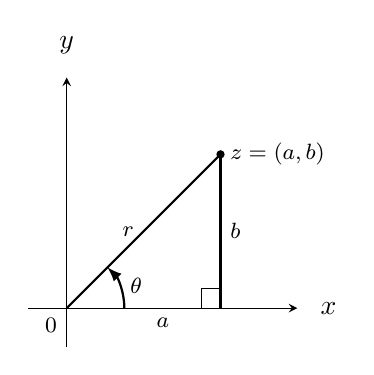
\begin{tikzpicture}
\begin{axis}[disabledatascaling, 
	clip mode=individual, 
    width=5cm, 
    height=5cm, 
    xlabel={$x$}, 
    ylabel={$y$}, 
    axis lines=middle, 
    xtick=\empty, 
    ytick=\empty, 
    xticklabels=\empty, 
    yticklabels=\empty, 
    every axis x label/.style={
      at={(ticklabel* cs:1.05)},
      anchor=west,
    },
    every axis y label/.style={
      at={(ticklabel* cs:1.05)},
      anchor=south,
    },
    domain=-5:5, 
    samples=100, 
    xmin=-0.5, 
    xmax=3, 
    ymin=-0.5, 
    ymax=3]
\draw[thick](0,0)--(2,2);
\fill[black] (2,2) circle (1.5pt);
\draw[thick,-latex] (0.75,0) arc [start angle=0,end angle=45,radius=0.75] node[right,text=black,font=\footnotesize,midway]{$\theta$};
\draw[thick](2,0)--(2,2);
\draw (1.75,0)--(1.75,0.25)--(2,0.25);
\node[below left,font=\footnotesize] at (0,0){$0$};
\node[below,font=\footnotesize] at (1.25,0){$a$};
\node[right,font=\footnotesize] at (2,1){$b$};
\node[left,font=\footnotesize] at (1,1){$r$};
\node[right,font=\footnotesize] at (2,2){$z=(a,b)$};
\end{axis} 
\end{tikzpicture}
